\chapter{System beskrivelse}
System er beregnet til behandling af patienter med acute ischemic stroke(AIS). Formålet er pre, per og postkonditioning af disse patienter. Systemet skal kunne lave arteriel okklusion i de øverste ydre ekstremiteter. For at sikre tilstrækkelig okklusion, skal det systoliske blodtryk først måles og derefter pumpe manchetten op til plus 25 mmHg over det målte tryk. Som minimum skal der afklemmes med et tryk på 180 mmHg. Okklusionenfasen  bliver holdt konstant i 5 minutter, hvorefter trykket lukkes ud der holdes en "pause" på 5 minutter, deflasionfasen. Denne process gentages indtil det antal specificeret cyklusser er kørt. Endvidere kræves der af produktet at både længden og antallet af okklusionfasen og deflasionfasen skal kunne ændres løbende. 
For at sikre at den arterielle afklemning ikke skader patienten, skal produktet kunne indikere om der opnås tilfredsstillende perfusion af det afklemte væv efter okklusionfasen. Produktet indbefatter derfor også et pulsoximeter, der efter hver afklemning tjekker kredsløbet. Systemet skal også kunne dokumenterer behandlingsforløbene, derfor udstyres systemet med ekstern hukommelse, der gør det muligt for bruger at eksportere dataen og se oversigt over forløbet. 
Som sideløbende krav kan produktet også bruges til okklusionstræning. Her pumpes manchet trykket op til 100 mmHg og det tryk holdes konstant indtil okklusionsættet er færdigt.  

\section{Systemoversigt}
\begin{figure}[H]
	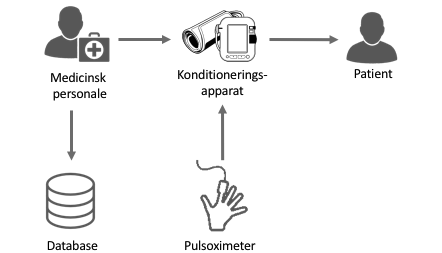
\includegraphics[width=0.8\textwidth]{Illustrationer/saelgertegning.png}
	\caption{Oversigt over systemet \textit{Konditioneringsapparat}}
\end{figure}
